\documentclass[17pt]{beamer}
\usetheme{Berkeley}
\usepackage{graphicx}

\title{Moogle}
\author{Daniel Amaranto Mares Garcia}
\date{\today}

\begin{document}

\begin{frame}
\titlepage
\end{frame}

\begin{frame}
\frametitle{Composición del Moogle}
\subsection*{Clases Principales}
\begin{itemize}
    
    \item Load 
    \item Matriz
    \item Consulta      
    \end{itemize}
    \end{frame}

\begin{frame}
\frametitle{Clase Load}
\subsection*{Clase Load}
\begin{itemize}
    \item[] \textbf{Campos o Atributos}
    \item private static string [] path=Directory.GetFiles(Path.Join(”..”,”Content”,””));
    \item private static string [][] text=new string[title.Length][];
    \item private static string[] title= new string[path.Length];
\end{itemize}
\end{frame}
\begin{frame}
\frametitle{Clase Load}
\begin{itemize}
    \item[] \textbf{Métodos o Funciones}
    \item public static void run ();
    \item public static string EliminarTildes( string texto);
    \item public static string EliminarCaracteres(string texto);
 \end{itemize}
\end{frame}
    
 \begin{frame}
    \frametitle{Clase Load}
    \begin{itemize}
        \item[] \textbf{Métodos o Funciones}
    \item public static string[][] GetText();
    \item public static string[] GetTitle();
    \item public static string [] GetPath();
    \end{itemize}
 \end{frame}
 \begin{frame}
    \frametitle{Clase Load}
    \begin{footnotesize}
        \fontsize{12}{10}
        La función principal de esta clase es cargar y modificar toda la base de
        datos (compuesta por archivos .txt), mediante el método run().
        \linebreak
        Dentro de este método se le asignan valores a todos los campos de clase excepto al
        path, y se realiza una llamada a los métodos EliminarTildes(string texto),
        EliminarCaracteres(string texto), los cuales modifican correspondientemente
        todos los archivos .txt  
    \end{footnotesize}
  \end{frame}
  \begin{frame}
    \frametitle{Clase Load}
    \textbf{Método run()}
    \begin{figure}[h]
    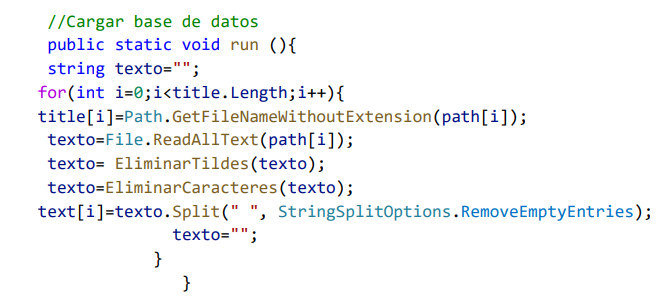
\includegraphics[width=11cm]{Code 1.png}
    \end{figure}
   \end{frame}
   \begin{frame}
    \frametitle{Clase Matriz}
    \subsection*{Clase Matriz}
    \begin{itemize}
        \item[] \textbf{Campos o Atributos}
        \item public static List ListDiccionarios;
        \item public static List ListDiccionariosTF;
        \end{itemize}
   \end{frame}
   \begin{frame}
    \frametitle{Clase Matriz}
    \begin{itemize}
        \item[] \textbf{Métodos o Funciones}
        \item private static void Diccionario();
        \item public static void DiccionarioTF();
        \item public static float Tf (float repeticion, float cantPalabras );
      \end{itemize}
       \end{frame}
        \begin{frame}
            \frametitle{Clase Matriz}
            \begin{itemize}
        \item[] \textbf{Métodos o Funciones} 
        \item public static float Idf (float TotalDocumentos, float documentos);
        \end{itemize}
        \begin{itemize}
            \item[] \textbf{Métodos Algebraicos}
            \item public static int [,] MultiplicarEscalar(int[,]a,int k);
            \end{itemize}
            \end{frame}
        
   
   \begin{frame}
    \frametitle{Clase Matriz}
    \begin{itemize}
        \item[] \textbf{Métodos Algebraicos}
          \item public static int[,] Sumar(int[,]a,int[,]b); 
        \item public static int[,] Restar(int[,]a,int[,]b); 
        \item static int[,] Multiplicar(int[,]a,int[,]b); 
    \end{itemize}
\end{frame}

    \begin{frame}
        \frametitle{Clase Matriz}
        \begin{itemize}
            \item[] \textbf{Métodos Algebraicos}
            \item public static int[,] Traspuesta(int[,]a);
        \end{itemize}
        \begin{figure}
            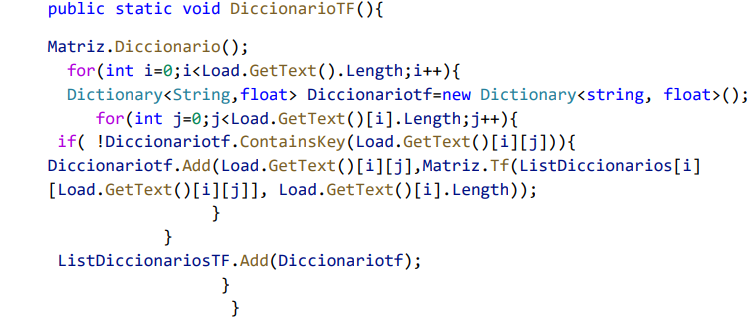
\includegraphics[width=9cm]{code 2.png}
        \end{figure}
    \end{frame}
    \begin{frame}
        \frametitle{Clase Consulta}
        \subsection*{Clase Consulta}
        \begin{itemize}
            \item[] \textbf{Campos o Atributos}
            \item public static string [] busqueda;
            \item public static float [] idf;
            \item public static float[] score =new float[Matriz.ListDiccionariosTF.
            Count];
         \end{itemize}
    \end{frame}
    \begin{frame}
        \frametitle{Clase Consulta}
        \begin{itemize}
            \item[] \textbf{Campos o Atributos}
            \item public static Dictionary Diccionariotfidf;
            \item public static string[] Docs=new string[3];
            \item  public static string[] snippet=new string[3];
         \end{itemize}
         \end{frame}
         \begin{frame}
\frametitle{Clase Consulta}
\begin{itemize}
    \item[] \textbf{Métodos o Funciones}
 \item public static void Modificar(string query);
 \item private static void SearchIdf();
\item private static void TfIdf ();
\item public static void DocsResultantes();
  \end{itemize}
 \end{frame}
 \begin{frame}
    \frametitle{Clase Consulta}
\begin{itemize}
    \item[] \textbf{Métodos o Funciones}
    \item public static bool show();
    \item public static void Importancia(string query);
    \item public static void Snippet();
     \end{itemize}
   \end{frame}
   \begin{frame}
    \frametitle{Clase Consulta}
    \begin{figure}
        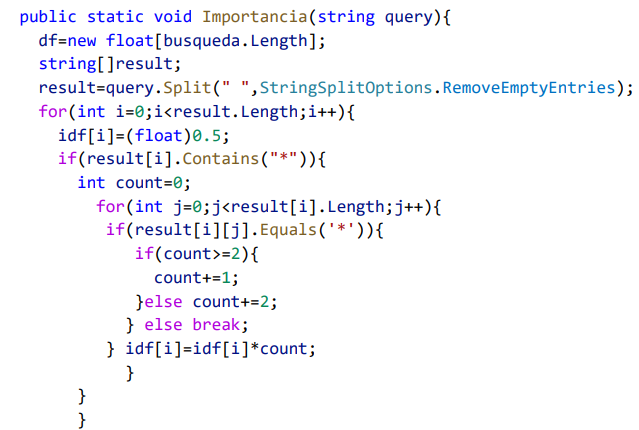
\includegraphics[width=9cm]{code 6.png}
    \end{figure}
 
    
 
 \end{frame}


    


    


\end{document}


 
